

\documentclass[11pt]{article}								% [Font size]{Type of document}


\usepackage[textwidth=17cm,textheight=24cm]{geometry}			% See geometry.pdf to learn the layout options. There are lots.
\geometry{a4paper}                      							% ... or a4paper or a5paper or ... 
\usepackage{graphicx}									% Package for including graphics 
%\usepackage{amssymb}									% American Mathematical Society Symbols and fonts
\usepackage{epstopdf}									% Conversion of eps to pdf files 
%\usepackage{hyperref}     									% Hyper text links in document and to external URLs
\usepackage[left=0.70cm, right=0.70cm, top=0.70cm, bottom=0.70cm]{geometry} % sort out the too large LaTeX default margins.
%\usepackage{graphicx} %for importing graphics, see \begin{figure} below.
\usepackage{amssymb,amsmath} % add some standard packages for maths and symbols
\usepackage[colorlinks=true,linkcolor=blue]{hyperref}

\linespread{1.5} 										% Single, Double, 1.5 line spacing, just put in the factor, here it is 1.5 times normal spacing


\DeclareGraphicsRule{.tif}{png}{.png}{`convert #1 `dirname #1`/`basename #1 .tif`.png}

\title{PH2150 Final Project Report - Fourier Series GUI}
\author{Candidate number: 1808666}
\date{\today}                                      							% Activate to display a given date or no date

\begin{document}
\maketitle
%%%%%%%%%%%%%%%%%%%%%%%%%%%%%%%%%%%%%%
\section{Demonstrating Fourier series \label{sec:section1}}
The GUI demonstrates how a Fourier series approximation of a square wave signal changes with different time periods and harmonics for a pre-determined range of $x$ values. The home page Figure 1 contains buttons which can be used to navigate between different pages within the GUI. There is another button to open this report. These pages contain concise pieces of information on different aspects of the Fourier series approximation, and a plotting page which contains the canvas where the plots appear.
\begin{figure}[ht]
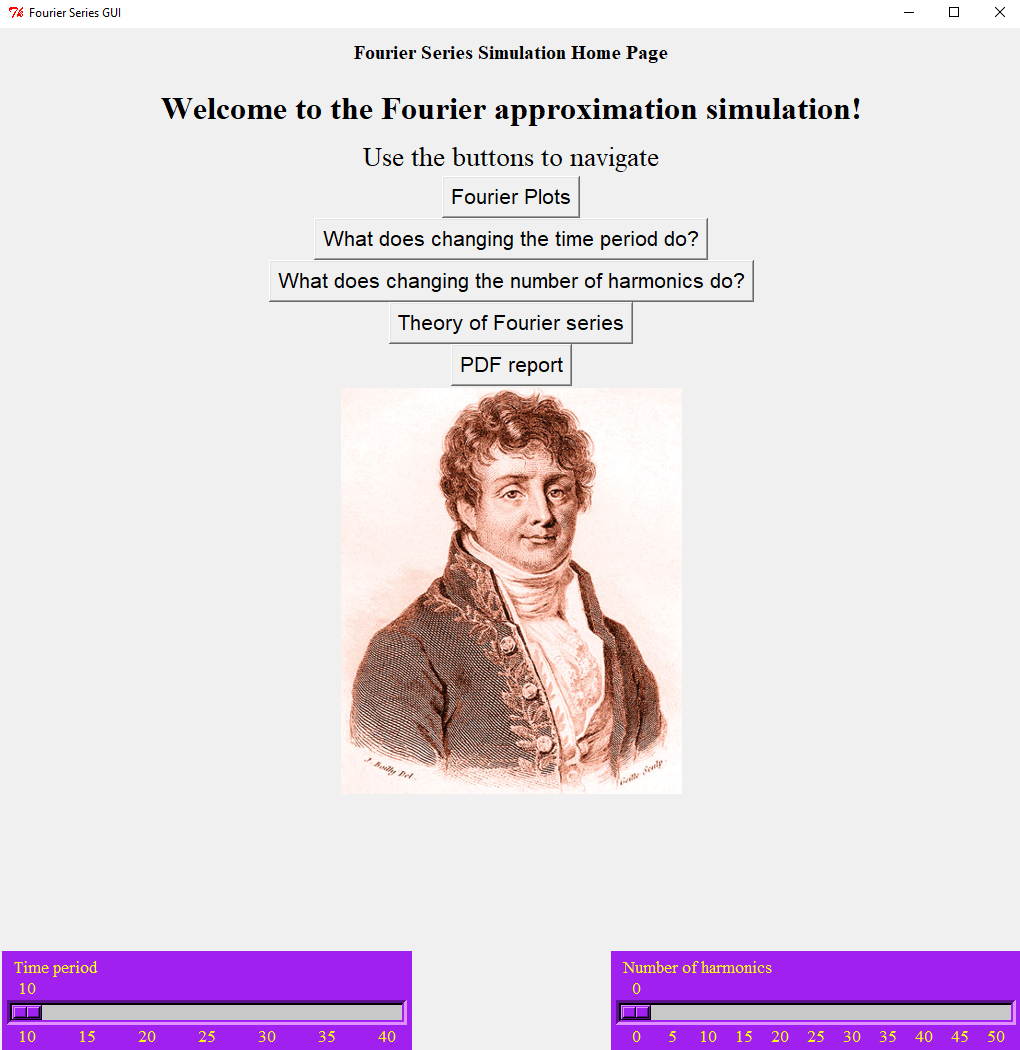
\includegraphics[width=9cm, height=6cm]{home_page3}
\centering
\caption{\emph{This is the home page that the user sees when the GUI is first launched. It contains the  buttons to navigate to other pages, and a welcoming picture of Joseph Fourier.}}
\label{fig:homepg}
\end{figure}
\begin{figure}[ht]
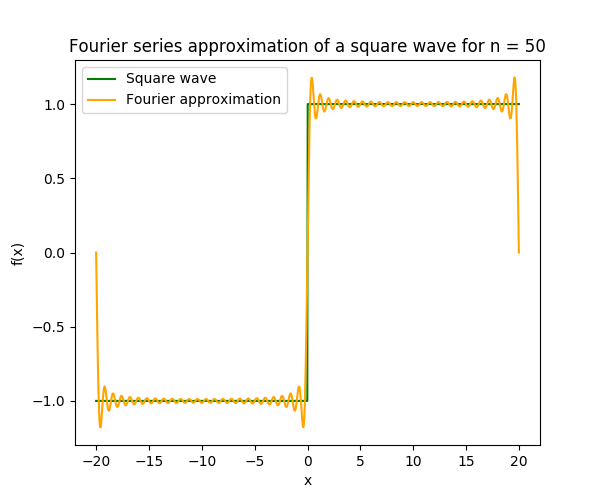
\includegraphics[width=9cm, height=6cm]{large_values1}
\centering
\caption{\emph{An example of using larger values within the sliders' ranges. This produces less cycles on the display due to the large time period, and a more accurate Fourier approximation due to the large number of harmonics. The Gibbs phenomenon is most evident for large numbers of harmonics. Here $T$ = 40, $n$ = 50.}}
\end{figure}
\begin{figure}[ht]
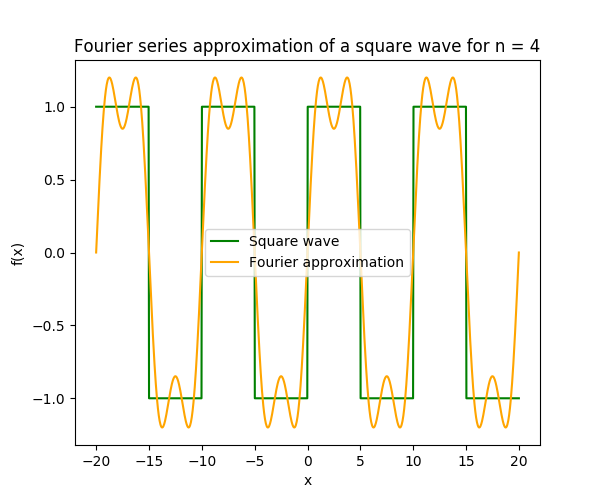
\includegraphics[width=9cm, height=6cm]{small_values1}
\centering
\caption{\emph{An example of using smaller values within the sliders' ranges. This produces more cycles on the display and an inaccurate Fourier approximation of the square wave signal. The Gibbs phenomenon is difficult to see with such a small number of harmonics. Here $T$ = 10, $n$ = 4.}}
\end{figure}
%%%%%%%%%%%%%%%%%%%%%%%%%%%%%%%%%%%%%%
\section{Mathematical modelling for a square wave approximation\label{sec:section2}}
The Fourier approximation consists of three individual components which are summed together to produce a series representation. The three components are the two Fourier coefficients, $a_{n}$ and $b_{n}$ and the average value of the function, $a_{0}$. Each of these components depend on the function $f(x)$ that defines the square wave signal. Square wave signals are physical representations of piecewise functions that have two components. 
\begin{equation}
\[
  f(x) =
  \begin{cases}
                                   1 & \text{ $0<x\leq\frac{T}{2}$} \\
                                   -1 & \text{ $\frac{T}{2}<x\leq T$} \\
  \end{cases}
\]
\label{eq:piecewise}
\end{equation}
\ref{eq:piecewise} is the simple function that was chosen to model the square wave in this GUI.
The function is defined in the range $-20\leq x\leq 20$ which was implemented using \emph{linspace}.

The $a_{0}$ and $a_{n}$ components of Fourier series are as follows
\begin{equation}
\begin{displaymath}
a_{0} = \frac{1}{L}\int_{-L}^{L} f(x) dx \;\; 
\label{eq:a0coeff}
\end{displaymath}
\end{equation}
\begin{equation}
\begin{displaymath}
a_{n} = \frac{1}{L}\int_{-L}^{L} \cos\bigg(\frac{n\pi x}{L}\bigg) f(x) dx \;\; 
\end{displaymath}
\label{eq:ancoeff}
\end{equation}
Given that, as mentioned earlier, $a_{0}$ is equivalent to the average value of $f(x)$, and noticing that the function is odd and symmetrical, the average value, and therefore $a_{0}$, is equal to zero.
The rule for odd functions also applies to all $a_{n}$ coefficients, which means they are also equal to zero so do not need to be calculated.
The third compnonent, Fourier coefficient $b_{n}$ is given by
\begin{equation}
\begin{displaymath}
b_{n} = \frac{1}{L}\int_{-L}^{L} \sin\bigg(\frac{n\pi x}{L}\bigg) f(x) dx \;\; 
\end{displaymath}
\label{eq:bncoeff}
\end{equation}
For odd functions, all $b_{n}$ have non-zero values, so are included in the series approximation;
\begin{equation}
\begin{displaymath}
f(x) = \frac{1}{2}a_{0} +  \sum_{n=1}^{\infty} a_{n} \cos\bigg(\frac{n\pi x}{L}\bigg) +  \sum_{n=1}^{\infty} b_{n} \sin\bigg(\frac{n\pi x}{L}\bigg) \;\
\end{displaymath}
\label{eq:fourierseries}
\end{equation}
\ref{eq:fourierseries} is the expression which sums all of the components together, producing the Fourier series. In this instance, it can be simplified to
\begin{equation}
\begin{displaymath}
f(x) = \sum_{n=1}^{\infty} b_{n} \sin\bigg(\frac{n\pi x}{L}\bigg) \;\
\end{displaymath}
\label{eq:fourierseriessimp}
\end{equation}
because $a_{0}$ = $a_{n}$ = 0.
%%%%%%%%%%%%%%%%%%%%%%%%%%%%%%%%%%%%%%
\section{Functionality \label{sec:section3}}
The plots are produced on the 'Fourier Plots' page, which is where the canvas is, as shown in Figure 4. Values for the time period $T$ and the number of harmonics $n$ are chosen from the sliders at the bottom of the page. These sliders have upper and lower limits so extreme values that could potentially break the program are not accessible. Once these values are chosen, the 'PLOT' button is pressed to display the result. This can be pressed more than once to overlap plots, or 'CLEAR' could be pressed to clear the axes. The 'Back' button appears on each page other than the home page and allows the user to navigate back to the home page.
\begin{figure}[ht]
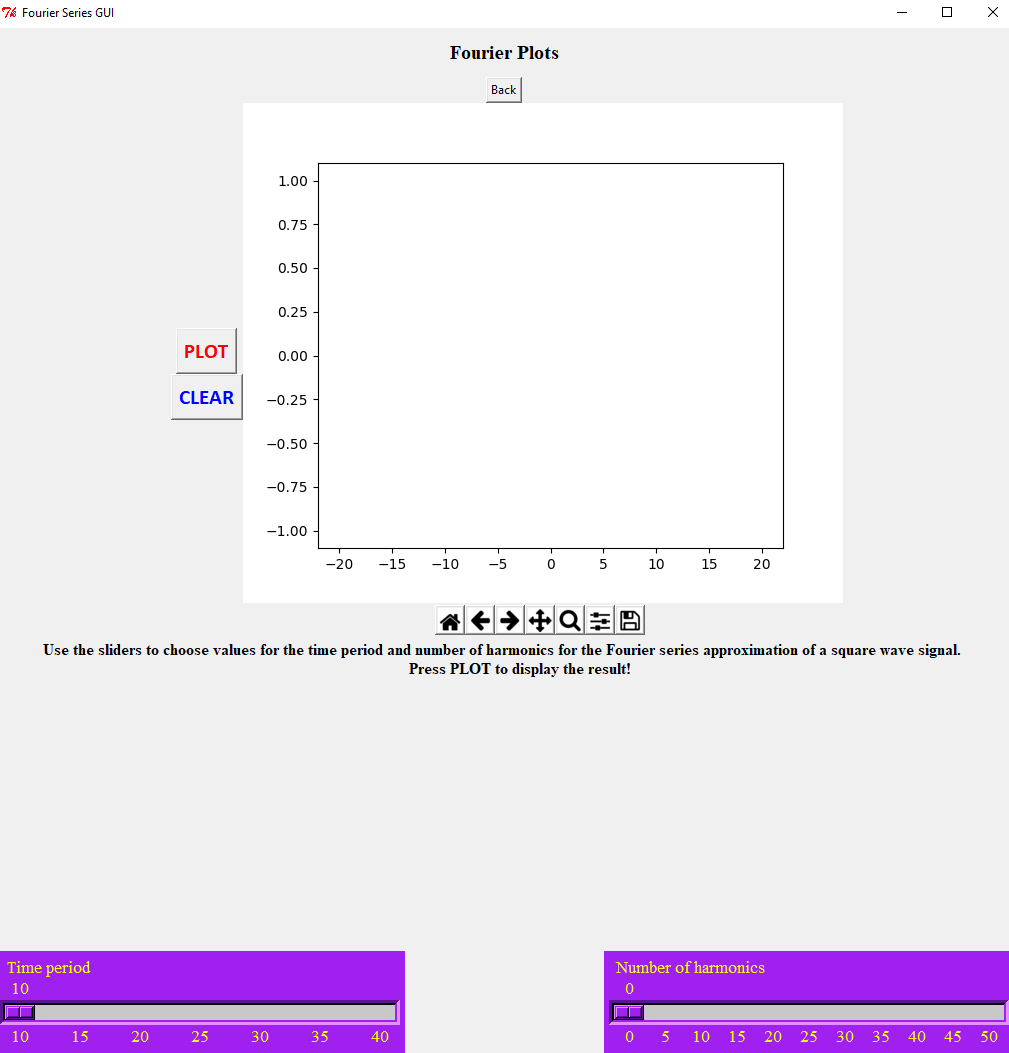
\includegraphics[width=9cm, height=6cm]{plot_page}
\centering
\caption{\emph{This is the page where the canvas is, and where the plots are displayed.}}
\label{fig:plotpg}
\end{figure}
The pieces of information on the other pages are imported as images of PDF files that were formatted using LaTeX to produce the most elegant looking equations, demonstrated in Figure 5.
\begin{figure}[ht]
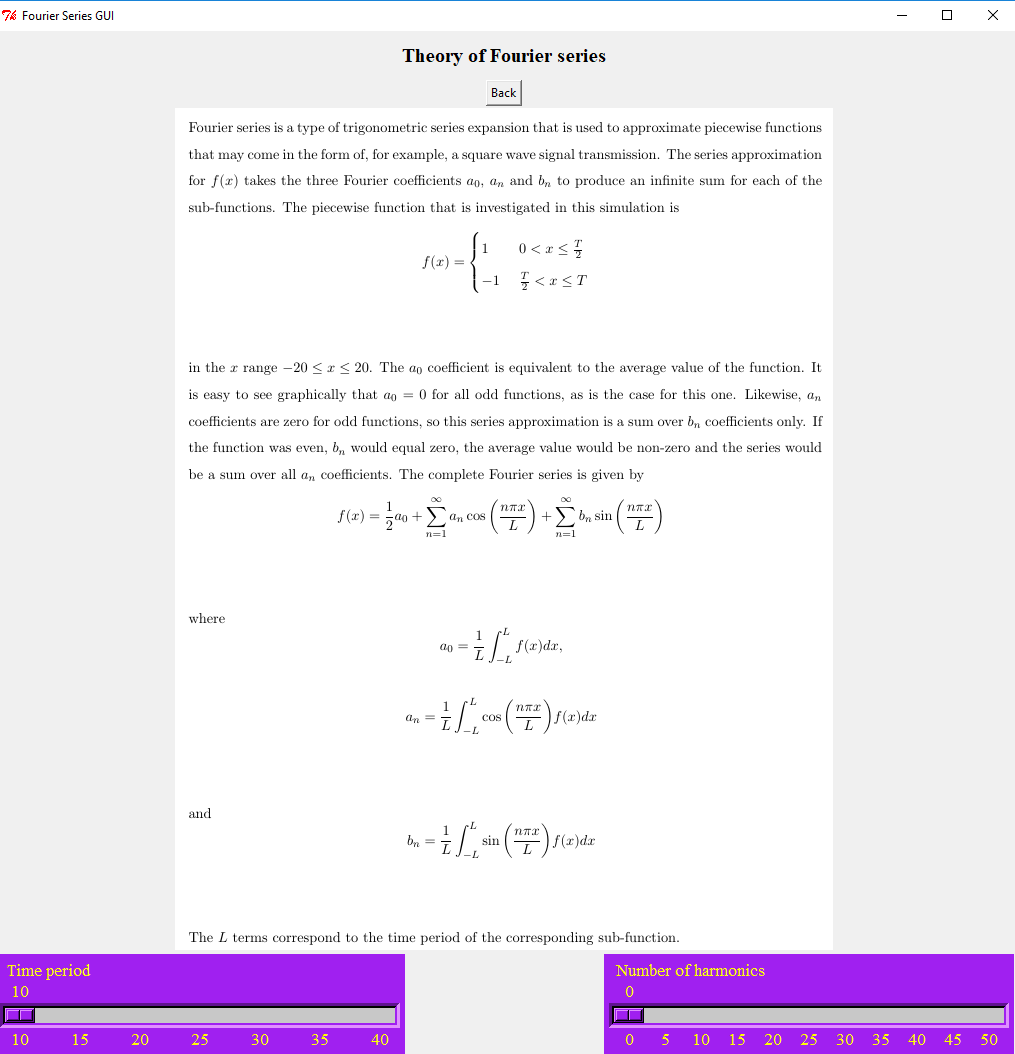
\includegraphics[width=9cm, height=6cm]{ft_page}
\centering
\caption{\emph{This is the home page that contains background information on Fourier series theory. An example of using LaTeX to produce the best formatting.}}
\label{fig:ftpg}
\end{figure}
%%%%%%%%%%%%%%%%%%%%%%%%%%%%%%%%%%%%%%



\begin{thebibliography}{widest-label}
\bibitem{latex} WolframMathWorld \url{http://mathworld.wolfram.com/FourierSeries.html}

\end{thebibliography}


\end{document}  